\documentclass[11pt]{article}

% ---------------- Packages ----------------
\usepackage{amsmath,amssymb,amsthm}
\usepackage{graphicx}
\usepackage{booktabs}
\usepackage{hyperref}
\usepackage{tikz}
\usepackage{algorithm}
\usepackage{algpseudocode}
\usetikzlibrary{arrows.meta, positioning, calc, fit}

% ---------------- Metadata ----------------
\title{DeltaSort: Fast incremental repair of sorted arrays under sparse updates}
\author{
  Shubham Dwivedi \\
  Independent Researcher \\
  \texttt{shubd3@gmail.com}
}
\date{\today}

\begin{document}
\maketitle

% ---------------- Abstract ----------------
\begin{abstract}
Maintaining sorted order under incremental updates is a common requirement in
practical systems, including user interfaces that render large sorted lists and
data-processing pipelines that consume streaming or change-data-capture updates.
In such settings, updates often arrive in small batches, and the set of modified
elements is explicitly known. Despite this, production systems frequently re-sort
entire arrays from scratch, ignoring available update locality.

This paper presents \emph{DeltaSort}, an incremental algorithm for restoring sorted
order in arrays under sparse, known updates. DeltaSort exploits explicit knowledge
of modified indices to reduce comparison costs and avoid unnecessary reordering.
The algorithm operates by reinserting updated values and locally repairing order
violations within bounded segments. An empirical evaluation in JavaScript shows
that DeltaSort substantially reduces comparator invocations and can outperform
native sorting for sufficiently small update volumes, particularly when comparison
functions are expensive. Limitations and directions for future work are discussed.
\end{abstract}

% ---------------- Introduction ----------------
\section{Introduction}

Sorted sequences are a foundational abstraction in software systems. User
interfaces frequently render large sorted lists, such as tables or feeds, while
data-processing systems maintain ordered views over continuously changing data.
In many of these systems, updates are incremental: only a small subset of elements
changes between successive evaluations, and the set of modified elements is often
explicitly available.

Despite this, a common practice is to re-sort the entire collection on each update.
This approach discards valuable information about update locality and can be
computationally wasteful, particularly when sorting involves expensive comparison
logic or when the data volume is large.

This paper explores a simple question: \emph{if the indices of modified elements
are known, can sorted order be restored more efficiently than by re-sorting from
scratch?}

DeltaSort addresses this question by formulating sorting under sparse updates as a
\emph{repair} problem rather than a full recomputation. The algorithm incrementally
restores order by resolving only those local violations induced by updates, while
leaving unaffected regions untouched. Although the approach is general, this work
focuses on in-memory arrays and does not attempt to integrate with database query
planners or storage engines.

The primary contribution of this paper is an algorithmic mechanism and an empirical
evaluation demonstrating that explicit update knowledge can materially change the
cost structure of sorting under realistic workloads.

% ---------------- Problem Definition ----------------
\section{Problem Definition}

Let $A$ be an array of length $n$ that was previously sorted under a stable total
order comparator $\prec$. Let $D \subseteq \{0, \dots, n-1\}$ be a set of indices
whose values have changed arbitrarily since the last sort. All indices not in $D$
retain their original values.

The goal is to restore $A$ to a globally sorted order under $\prec$, preserving
stability, while exploiting knowledge of $D$ to reduce unnecessary work.

The problem differs from general sorting in two important ways:
\begin{itemize}
  \item The array is known to have been sorted prior to the updates.
  \item The set of modified indices is explicitly available.
\end{itemize}

DeltaSort is designed for scenarios in which $|D| \ll n$.

% ---------------- Algorithm Overview ----------------
\section{Algorithm Overview}

DeltaSort operates in three phases:
\begin{enumerate}
  \item \textbf{Dirty reinsertion.} Dirty indices are sorted, and the corresponding
        values are sorted and reinserted at their original positions.
  \item \textbf{Violation detection.} The array is scanned in order of dirty indices
        to identify local order violations.
  \item \textbf{Localized repair.} Each violation is resolved by moving the offending
        element into its correct position within a bounded segment using a stable
        shift operation.
\end{enumerate}

The algorithm avoids speculative movement and confines all repairs to the minimal
segment required to restore order.

\subsection{Algorithm}

Algorithm~\ref{alg:deltasort} presents the DeltaSort procedure. The algorithm
assumes that the input array was previously sorted and that the set of dirty
indices is explicitly known.

\begin{algorithm}[H]
\caption{DeltaSort}
\label{alg:deltasort}
\begin{algorithmic}[1]
\Require Array $A$ of length $n$, comparator $\prec$, dirty index set $D$
\Ensure $A$ restored to sorted order under $\prec$

\State $I \gets$ sorted list of indices in $D$
\State $V \gets$ values $\{A[i] \mid i \in I\}$ sorted under $\prec$
\For{$k \gets 0$ to $|I|-1$}
    \State $A[I[k]] \gets V[k]$
\EndFor

\State $S \gets$ empty stack \Comment{Pending right-moving or stable indices}
\State $leftBound \gets 0$

\For{each $i \in I$ in increasing order}
    \State $dir \gets$ \Call{Direction}{$A, i, \prec$}
    \If{$dir = R$ or $dir = S$}
        \State push $i$ onto $S$
    \Else \Comment{$dir = L$}
        \State $rightBound \gets i - 1$
        \While{$S$ not empty}
            \State $j \gets$ pop $S$
            \If{\Call{Direction}{$A, j, \prec$} $= R$}
                \State \Call{FixRight}{$A, j, leftBound, rightBound, \prec$}
            \EndIf
        \EndWhile
        \State \Call{FixLeft}{$A, i, leftBound, \prec$}
        \State $leftBound \gets$ new position of $A[i] + 1$
    \EndIf
\EndFor

\State $rightBound \gets n - 1$
\While{$S$ not empty}
    \State $j \gets$ pop $S$
    \If{\Call{Direction}{$A, j, \prec$} $= R$}
        \State \Call{FixRight}{$A, j, leftBound, rightBound, \prec$}
    \EndIf
\EndWhile
\end{algorithmic}
\end{algorithm}

% ---------------- Diagram: Array with Dirty Indices ----------------
\begin{figure}[h]
\centering
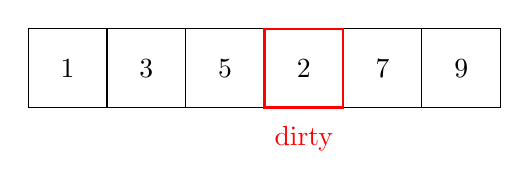
\begin{tikzpicture}
  \foreach \i/\v in {0/1,1/3,2/5,3/2,4/7,5/9} {
    \draw (\i,0) rectangle (\i+1,1);
    \node at (\i+0.5,0.5) {$\v$};
  }
  \draw[red, thick] (3,0) rectangle (4,1);
  \node[red] at (3.5,-0.4) {dirty};
\end{tikzpicture}
\caption{A previously sorted array with a single dirty index introducing a local violation.}
\end{figure}

% ---------------- Repair Mechanism ----------------
\subsection{Repair Mechanism}

When a local violation is detected, DeltaSort identifies the minimal feasible
segment within which the offending element can be repositioned without violating
sortedness or stability. A binary search determines the target position, and a
stable shift inserts the element directly into its final location.

This process is repeated until no violations remain.

% ---------------- Correctness ----------------
\section{Correctness}

The correctness of DeltaSort follows from three invariants maintained throughout
execution.

\paragraph{Invariant 1 (Sorted Clean Regions).}
All regions not containing unresolved dirty elements remain sorted at all times.

\paragraph{Invariant 2 (Segment Confinement).}
Each repair operation moves an element only within the minimal segment required
to restore order, and no element crosses a boundary that would violate sortedness
or stability.

\paragraph{Invariant 3 (Progress).}
Each repair operation strictly reduces the number of unresolved local violations.

\paragraph{Theorem.}
Upon termination, the array is globally sorted under $\prec$ and stability is
preserved.

\paragraph{Proof Sketch.}
By Invariant 3, the algorithm terminates after a finite number of repairs. By
Invariant 1, all unaffected regions remain sorted. By Invariant 2, no repair
introduces new violations outside its segment. At termination, no local violations
remain; therefore, no global violations exist. Stability is preserved by construction.
\qed

% ---------------- Evaluation ----------------
\section{Evaluation}

DeltaSort was implemented in JavaScript and evaluated against the native
\texttt{Array.prototype.sort} implementation. Two primary metrics were measured:
comparator invocations and wall-clock runtime.

Experiments were conducted on arrays ranging from $10^5$ to $10^6$ elements, with
varying proportions of dirty indices. For small update volumes, DeltaSort exhibits
a dramatic reduction in comparator calls and can outperform native sorting,
particularly when comparators are expensive.

% ---------------- Placeholder Chart ----------------
\begin{figure}[h]
\centering
\fbox{
  \parbox{0.8\linewidth}{
    \centering
    Placeholder for speedup vs.\ delta percentage plot.
  }
}
\caption{Runtime comparison between DeltaSort and native sorting as a function of update sparsity.}
\end{figure}

% ---------------- Limitations and Future Work ----------------
\section{Limitations and Future Work}

DeltaSort is not a general-purpose replacement for production sorting algorithms.
As update volume increases, memory movement costs dominate and native sorting
outperforms incremental repair. Additionally, this work does not address integration
with database storage engines or query optimizers.

Future work includes a formal correctness proof, tighter theoretical bounds on
movement costs, comparison against fully instrumented reference sorting algorithms,
and adaptive heuristics for selecting between DeltaSort and native sorting based
on observed update patterns.

% ---------------- Bibliography ----------------
\bibliographystyle{plain}
\nocite{*}
\bibliography{refs}

\end{document}